\chapter{Methods}

\paragraph{Problem Description}
Surgical robot navigation presents unique challenges, particularly when operating on soft, deformable organs. Unlike rigid environments, where a robot can rely on predefined maps and fixed obstacle positions, deformable organs continuously change shape due to external forces, physiological processes, and surgical interactions. This introduces uncertainty in navigation, making it difficult to plan and execute precise movements.

\paragraph{Key Challenges}
\begin{enumerate}
\item \textbf{Deformation of Organs:} Soft tissues can shift, stretch, or compress unpredictably, leading to non-static obstacles and pathways.
\item \textbf{Partial Observability:} Due to the limited field of view of endoscopic cameras, occlusions, and the dynamic nature of the surgical site, the robot does not have full knowledge of the environment at any given time.
\item \textbf{Real-Time Adaptation:} The robot must continuously update its navigation strategy based on incomplete and evolving sensory data.
\item \textbf{Safety Constraints:} Unlike traditional robotic navigation, errors in surgical settings can result in severe patient harm, requiring ultra-precise movement planning.
\end{enumerate}

\paragraph{POMDPs for Surgical Robot Navigation}
Given the challenges of deformable environments and partial observability, \glspl{pomdp} provide a suitable 
framework for modeling surgical robot navigation. A \gls{pomdp} extends a traditional \gls{mdp} by incorporating 
uncertainty in both state transitions and observations, making it ideal for scenarios where the robot 
does not have full knowledge of the environment at any given moment.

In a surgical context, the robot must estimate the underlying state of the organ based on noisy and 
limited sensory data. The \gls{pomdp} framework allows for probabilistic reasoning over possible 
states and dynamically updating beliefs based on new observations. This enables more robust 
decision-making under uncertainty, improving navigation efficiency and patient safety through uncertainty 
quantification.

\paragraph{Relation to a 2D Deformable Maze}
A simplified analogy can be drawn between surgical robot navigation and a robot navigating a 2D deformable maze. In this case:
\begin{itemize}
\item The \textbf{maze walls} represent anatomical structures that move and deform in real-time.
\item The \textbf{robot's sensors} are analogous to a surgical camera with a limited and dynamic field of view.
\item The \textbf{algorithm} must adapt to continuous environmental changes, rather than relying on a static map.
\item The \textbf{goal} is to reach a target point while avoiding dynamically shifting obstacles and ensuring efficient movement.
\end{itemize}

\paragraph{Relation to 3D Simulation of Surgical Manipulation of Soft Objects}
A crucial aspect of developing and validating surgical robot navigation algorithms is the use of 3D 
simulations of soft object manipulation. These simulations provide a controlled environment where the 
behavior of deformable tissues can be accurately modeled using finite element methods. 
By simulating realistic tissue deformations, forces, and interactions, we can test and 
refine robotic control strategies before deploying them in real-world surgical settings. Additionally, 
3D simulations enable the integration of sensory feedback loops, allowing for the evaluation of 
different perception and decision-making strategies under conditions of uncertainty.\\


This analogy highlights the importance of real-time sensing, dynamic path planning, and uncertainty 
management in both surgical robotics and general deformable environment navigation. 
Future advancements in soft-tissue modeling, AI-driven prediction, and sensor fusion will be 
crucial in improving the efficacy of surgical robot navigation under these constraints.


We adopted a bottom up approach, increasing the complexity of the task in increasingly complex environments.
Our objective is to explore the applicability of \gls{rl} and \glspl{pomdp} to navigation and manipulation 
in deformable environments related to the surgical tasks.

In the following we assumied the model of the environment to be known or learnable, 
given the preoperative imaging medical data. This would allow us to model 
the problem as a \gls{pomdp} and apply the methods described in previous chapters.


\section{Gridworld}
The first task we consider is a simple gridworld, where the agent had to navigate from a random 
starting position to a goal position. The twist is given by the deformable property of the environment.

\paragraph{State Space}

The environment is a 2D grid of size $30 \times 30$ where each cell can be either empty or occupied by an obstacle.
the state is represented as a tuple $(x,y,\phi, \theta)$ where $x$ and $y$ are the discrete coordinates of the agent in the grid, 
$\phi$ is the orientation of the agent (it can point up, down, right, or left) and $\theta$ is a parameter controlling the linear scale deformation  
relative to $xy$ axis for a total of 81 discrete deformations.
We assume perfect observability upon the agent's position and orientation while the deformable property 
of the environment has to be estimated through observations. This is done to reflect the clinical setting where the preoperative 
imaging data is available but the intraoperatory setting might be different due to the deformation of the
organs and tissues. 

\begin{figure}[H]
    \centering
    \begin{subfigure}{0.45\textwidth}
        \centering
        
\includegraphics[width=0.75\linewidth]{images/gridworld_5x8.png}
        \caption{$\theta$ = (5,8)}
    \end{subfigure}
    \hfill
    \begin{subfigure}{0.45\textwidth}
        \centering
        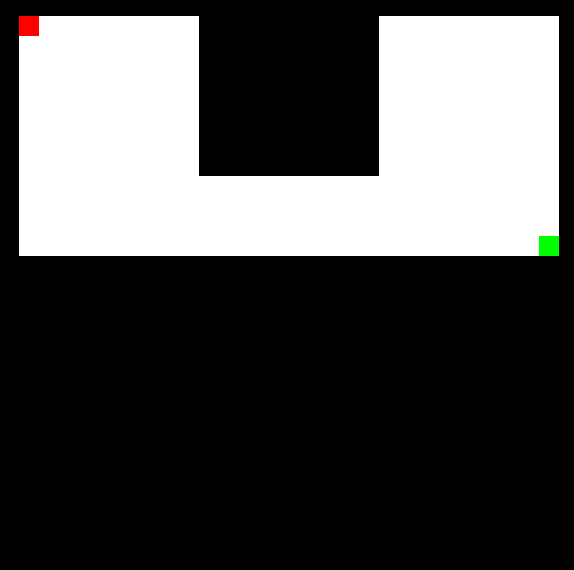
\includegraphics[width=0.75\linewidth]{images/gridworld_9x4.png.png}
        \caption{$\theta$ = (9,4)}
    \end{subfigure}
    \caption{Gridworld Environment for $s = (1,1,0,\theta$)}
    \label{fig:gridworld}
\end{figure}

Notice that the deformable property of the environment directly affects the target position (\cref{fig:gridworld}).

\paragraph{Action Space}

The agent can move in four directions: up, down, left, right. The action space is therefore $A = \{0,1,2,3\}$.

\paragraph{Observation Space}

Every time the agent moves, it receives an observation which corresponds to the type of adjacent cells 
in the grid $O = \set{o \in \set{0,1}^4 }$ where $0$ refers to an empty cell and $1$ to 
an obstacle (\cref{fig:observationgridworld}). 

\begin{figure}[H]
    \centering
    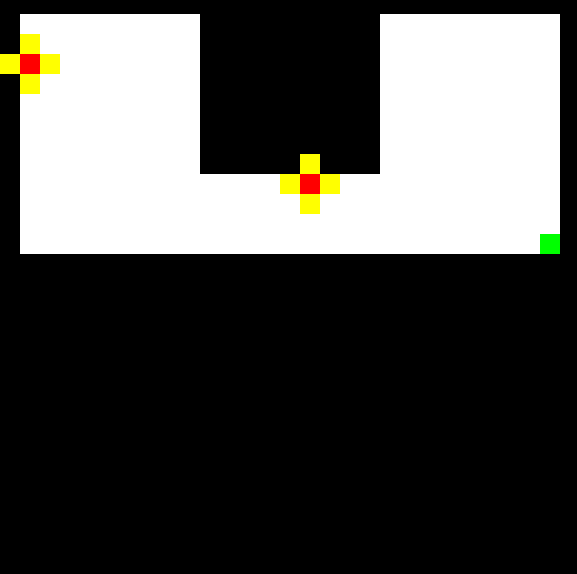
\includegraphics[scale=.25]{images/gridworld_observation.png}
    \caption{Observations in Gridworld}
    \label{fig:observationgridworld}
\end{figure}


\paragraph{Transition Function}
Always assuming deterministic transitions, the transition function is defined as follows:
$$\mathcal{T}(s'|s,a) =
\begin{cases}
    1 &   \text{if } s' \text{ is the result of applying action } a \text{ to state } s, \\
    0 &   \text{otherwise}. \\
\end{cases}
$$

In this simulation we assume that every transition that ends up inside the grid is a valid 
one. 
This is done to simplify the problem and focus on the deformable property only without 
the need to consider an elaborate transition model. The agent will nonetheless avoid 
obstacles if possible thanks to the reward structure.

\paragraph{Reward Function}

The reward function $\mathcal{R}(s,a,s')$ is defined as follows:


 $$\mathcal{R}(s,a,s') = 
    \begin{cases}
    \frac{-0.1}{mapsize} &   s' \neq s_{goal} \wedge \text{free cell}, \\ 
    \frac{-0.2}{mapsize} &   s' \neq s_{goal}  \wedge \text{hit wall},\\
    1 &   s' = s_{goal}. \\
    \end{cases}    
$$


\paragraph{Observation Function} The conditional observation probabilities $O(o|s,a)$ 
are also deterministic:
$$O(o|s,a)= O(o|s) = 
\begin{cases}
    1 &   \text{if } (x,y) \text{ adjacent cells for map } f_\theta(M) \text{are compatible with } o,\\
    0 &   \text{otherwise}. \\
\end{cases}
$$

where adjacent cells are defined as the cells in the 4 directions of the agent's orientation 
as in \cref{fig:observationgridworld}.

\paragraph{Belief State}
Because the agent does not directly observe the environment's state, the agent must make decisions under uncertainty of the true environment state. 
The general update rule for the belief state is given by the Bayes' rule.
Adapting it to the gridworld 
case, given the only source of uncertanty is only on the 
deformation parameter, the belief state is a probability distribution 
over possible deformations.
Denoting with $\psi = (x,y,\phi)$ the observable part of the state, the belief 
update collapses to belief over deformations since:

$$b(s) = b(x,y,\phi,\theta) = b(\psi, \theta) = \delta_{\psi} \cdot b(\theta)$$

where $\delta_{x,y,\phi}$ is $1$ if the agent is in position $(x,y)$ and orientation $\phi$ and $0$ otherwise.
By \cref{eq:beliefupdate} the belief update is then given by:

\begin{equation}
    \label{eq:beliefupdategridworld}
    b^{a,o}(\psi',\theta') = \eta O(o\mid \psi',\theta') \delta_{\psi'}b(\theta) 
\end{equation}

% \begin{cases}
%     \eta O(o\mid \psi',\theta')b(\psi,\theta) & \text{if } \mathcal{T}(s,a,s') = 1 \\
%     0 & \text{otherwise}.\\
% \end{cases}


\subsection{Tests}

Given the discrete nature of the deformations, we tested exact belief updates.
Traditional Value Iteration and Perseus Infotaxis

Deep q-learning 
Discrete update of the belief state is performed by the agent at each time step.


STATES: 236196
ACTIONS: 4
OBSERVATIONS: 16

maze size 30x30

\begin{table}[h]
\centering
\begin{tabular}{lcc}
\toprule
\textbf{Algorithm} & \textbf{Avg. Reward} & \textbf{Avg. Steps} \\
\midrule
MDP (upper bound) & -19.44 & 18.51\\
MLS & -26.47 & 23.93\\
TS &-26.13 & 24.231\\
QMDP & -24.71 & 23.75 \\
FIB & -25.49 & 23.55 \\
\bottomrule
\end{tabular}
\caption{Performance comparison of different algorithms on the Gridworld task. MDP represents the theoretical upper bound with perfect information.}
\label{tab:gridworld_results}
\end{table}

FIB and QMDP are equivalent given the formulation of the problem. stiamo soltanto 
testando l'imprecisione dell'observation model.


\section{Deformable Maze}
The second task was structured just like the first one increasing the environment complexity.
In this case we considered a continuous space and a continuous deformation parameter, 
keeping the discrete action space and observation space. This was done to provide 
a more insightful analysis of the possible scaling of the problem and techniques 
used to solve it.
   
\paragraph{State Space}
The environment is a continous 2D square of side length $1$.
the state is represented as a tuple $(x,y, \theta)$ where $x$ and $y$ are the Cartesian coordinates of the agent position, 
and $\theta$ is a parameter controlling the affine transformation: 
$$M_{\theta} = 
\begin{bmatrix}
\theta_{0,0} & \theta_{0,1} \\
\theta_{1,0} & \theta_{1,1}
\end{bmatrix}
$$  
where the diagonal elements range is $0.4 \leq \theta_{ii} \leq 1$ and the 
off-diagonal elements range is $-0.2 \leq \theta_{i\neq j} \leq 0.2$.
We assume perfect observability upon the agent's position while the deformable property 
of the environment has to be estimated through observations.

\begin{figure}[H]
    \centering
    \begin{subfigure}{0.45\textwidth}
        \centering
        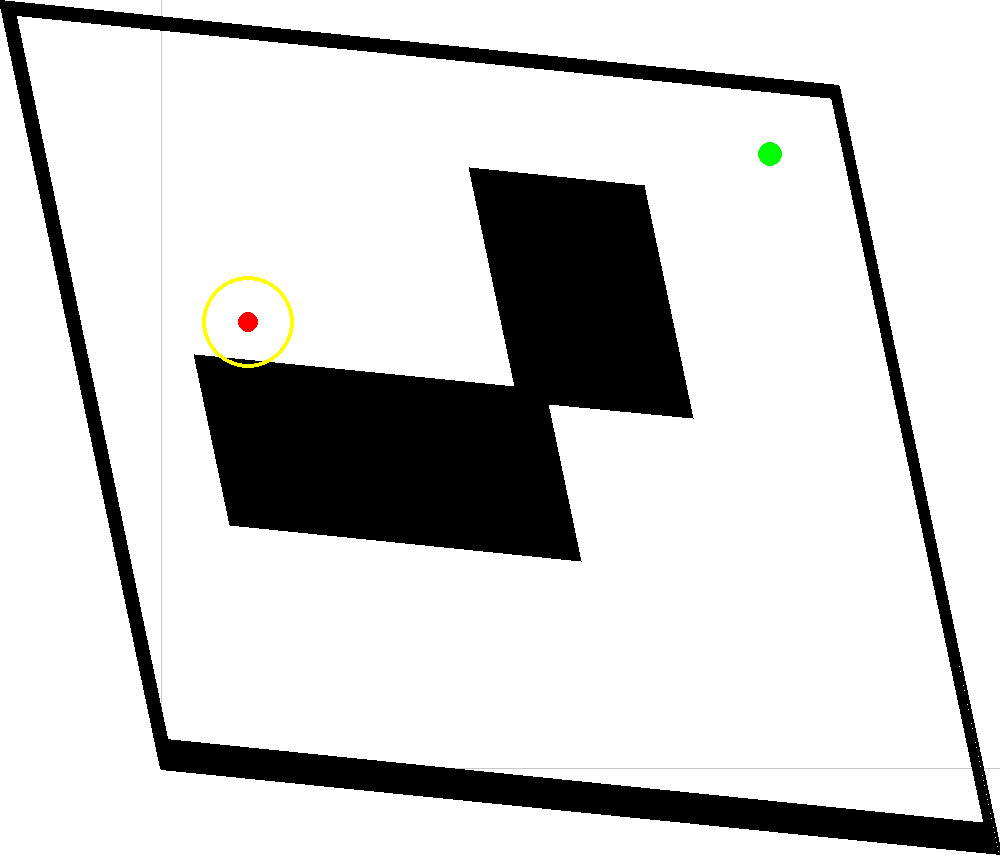
\includegraphics[width=0.55\linewidth]{images/maze_0.9_-0.17_-0.09_0.82.png}
        % \caption{$\theta$ = (5,8)}
    \end{subfigure}
    \hfill
    \begin{subfigure}{0.45\textwidth}
        \centering
        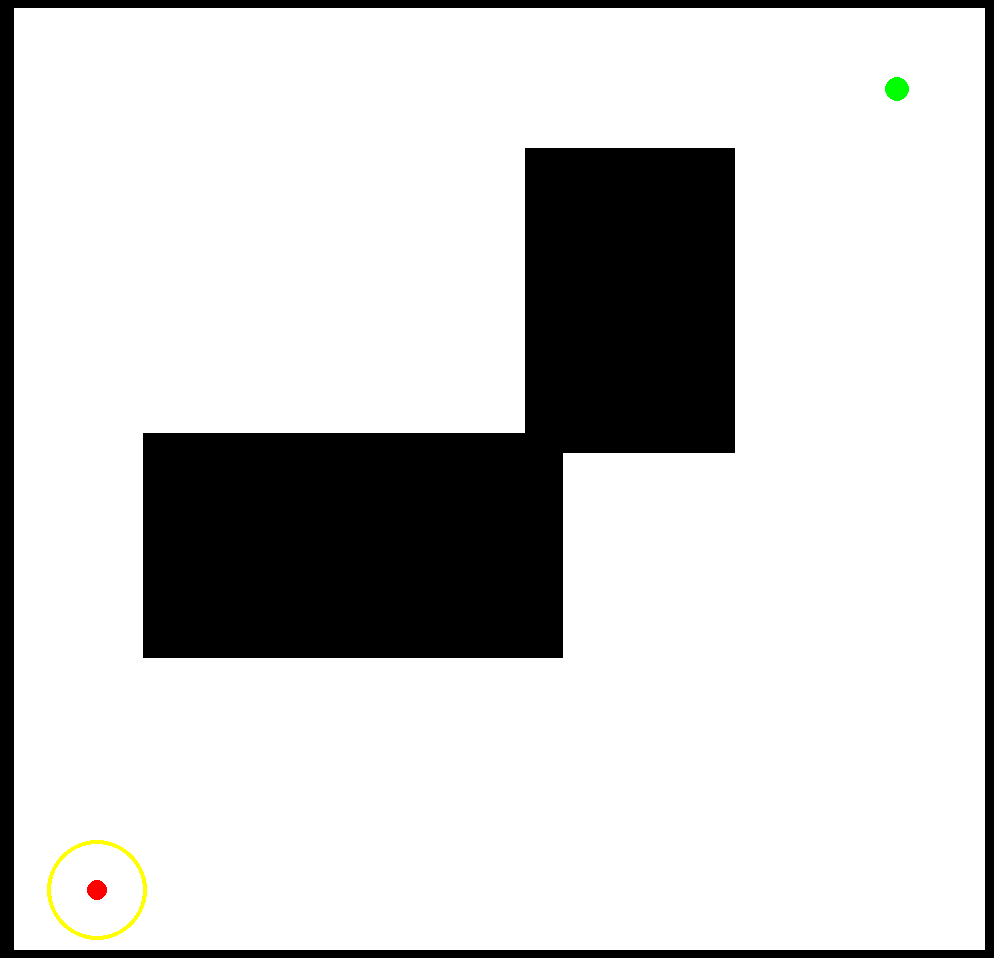
\includegraphics[width=0.55\linewidth]{images/maze_1.png}
        % \caption{$\theta = \mathcal{1}$}
    \end{subfigure}
    \hfill
    \begin{subfigure}{0.45\textwidth}
        \centering
        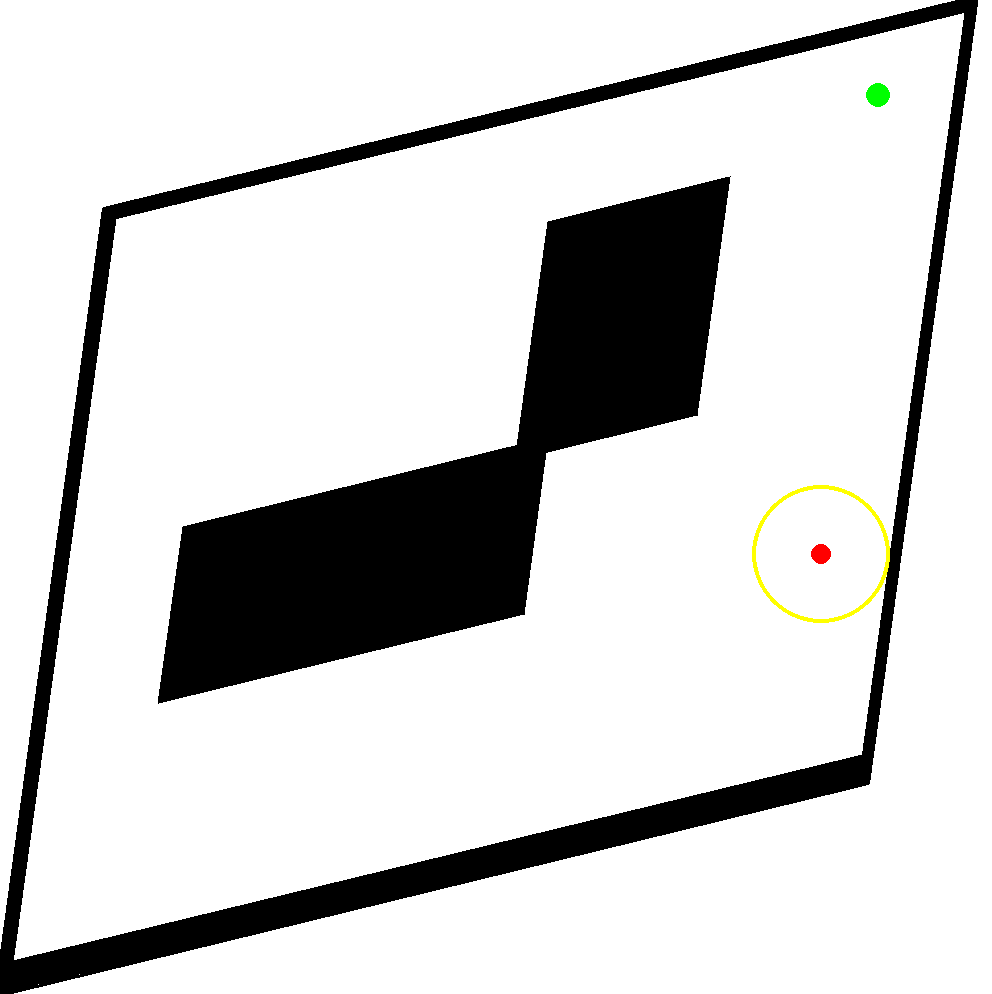
\includegraphics[width=0.55\linewidth]{images/maze_0.62_0.07_0.15_0.56.png}
        % \caption{$\theta$ = (9,4)}
    \end{subfigure}
    \caption{Maze Environment for different $\theta$}
    \label{fig:mazenv}
\end{figure}

\Cref{fig:mazenv} shows the agent (red) that observes the presence of obstacles (black) inside its 
    observtion radius (yellow) while trying to reach the goal (green).


\paragraph{Action Space}
Actions are the same as in the gridworld case, discrete movements of $stepsize =0.02$
in the four cardinal directions.

\paragraph{Observation Space} Observations are defined as elements of 
$O = \set{ o \in \set{ 0, 1 }^4 }$ where $0$ refers to an empty cell and $1$ to an 
obstacle. Obstacle presence is checked along cardinal directions N, S, E, W at any distance 
in the observation radius of the agent $r = 0.05$.

\paragraph{Transition Function}
Always assuming deterministic transitions, the transition function is defined as follows:
$$\mathcal{T}(s'|s,a) =
\begin{cases}
    1 &   \text{if } s' \text{ is the result of applying action } a \text{ to state } s, \\
    0 &   \text{otherwise}. \\
\end{cases}
$$
Analogous considerations to the gridworld case apply.

\paragraph{Reward Function}

The reward function $\mathcal{R}(s,a,s')$ is defined as follows:


 $$\mathcal{R}(s,a,s') = 
    \begin{cases}
    -1 &  s' \neq s_{goal} \wedge \text{free cell}, \\ 
    -2 & s' \neq s_{goal}  \wedge \text{hit wall or outside bounds},\\
    1  & s_{goal} \text{ in observation radius}. \\
    \end{cases}    
$$

\paragraph{Observation Function}
The conditional observation probabilities $O(o|s,a)$ 
are also deterministic:
$$O(o|s,a)= O(o|s) = 
\begin{cases}
    1 &   \text{if } (x,y) \text{ adjacent cells for map } f_\theta(M) \text{are compatible with } o,\\
    0 &   \text{otherwise}. \\
\end{cases}
$$

\subsection{Tests}

Given the continuous nature of the environment, we didn't consider value iteration or 
Perseus. We tested PPO and DQN on the belief space without success

DQN - PPO 
Belief update: dicrete variational inference laplace approximation particle filters 
Different observation informativity.

TS con 1000 particles
Mean episode Reward:  -29.4585
Mean number of steps:  43.746

\begin{table}[h]
    \centering
    \begin{tabular}{lccc}
    \toprule
    \textbf{Algorithm} & \textbf{Avg. Reward} & \textbf{Avg. Steps} & \textbf{Belief Update}\\
    \midrule
    MDP (upper bound) & -21.843 & 30.534 & None\\
    % QMDP & -24.715 & 23.75 \\
    MLS & -39.866 & 56.818  & Particles (2000)  \\
    TS & -28.491 & 43.474  & Particles (2000)  \\

    \bottomrule
    \end{tabular}
    \caption{Performance comparison of different algorithms on the Maze task averaged
    over 1000 episodes.}
    \label{tab:maze_results}
\end{table}
    

\section{Surgical Task}
We now move on to a different task that is more related to the surgical setting and
deformable object manipulation.


The environment is based on \cite{10.5555/3648699.3649067} and models a sub-task from laparoscopic cholecystectomy, i.e., 
the minimally invasive removal of the gallbladder. 
During dissection of the yellow gallbladder from the red liver, the blue
grasper has to grasp the distal end (infundibulum) of the partially 
resected gallbladder. Afterwards, the grasper retracts the gallbladder,
exposing a visual marker, which represents the point that should be
cut next. The green electrocautery hook then navigates to the visual
marker and activates in order to cut the tissue. The task is complete
when the target is visible to the camera and the cauter activates while
touching it (\cref{fig:surgicaltask}).
The task combines the challenges of grasping a deformable object, coordinating 
heterogeneous instruments, and performing multiple sequential steps to solve the task. Although
this task models cholecystectomy, the task of exposing
and then interacting with a region of interest often appears in surgical contexts.

\begin{figure}[H]
    \centering
    \begin{subfigure}{0.45\textwidth}
        \centering
        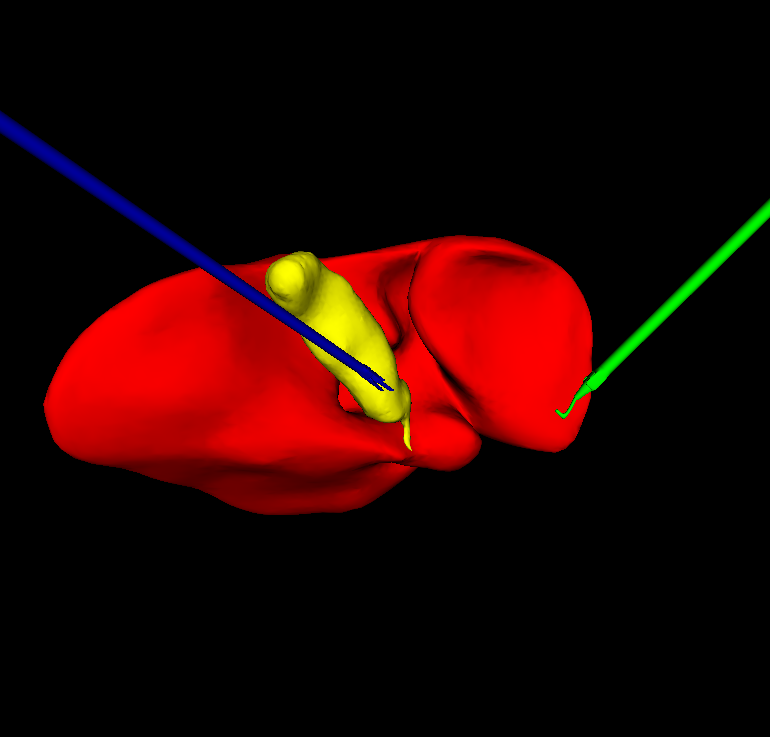
\includegraphics[width=0.75\linewidth]{images/grasplifttouch.png}
        \caption{Segmented}
    \end{subfigure}
    \hfill
    \begin{subfigure}{0.45\textwidth}
        \centering
        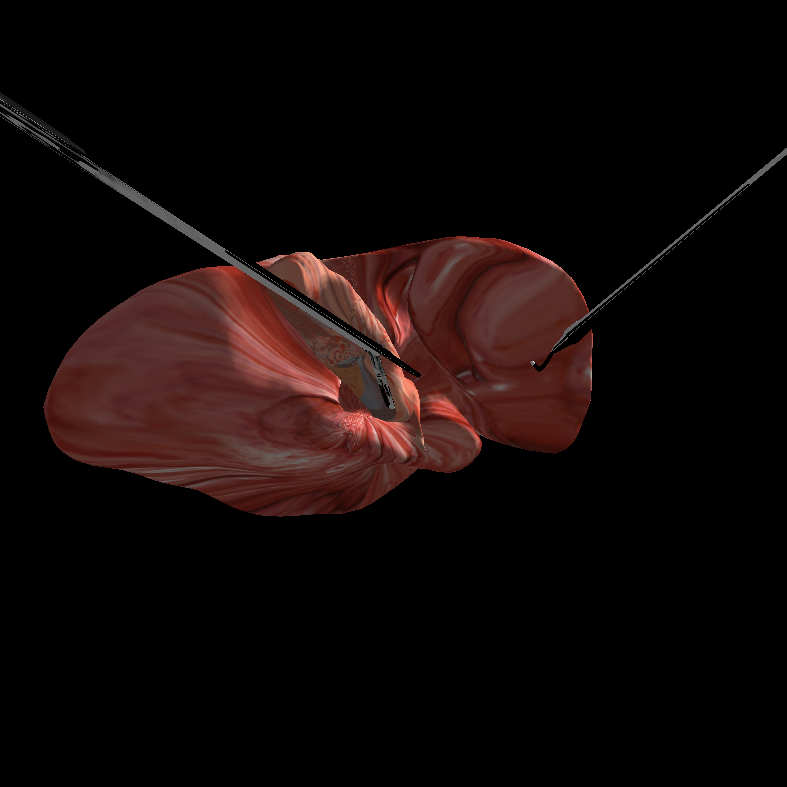
\includegraphics[width=0.72\linewidth]{images/grasplifttouch_real.png}
        \caption{Real}
    \end{subfigure}
    \caption{Surgical Environment}
    \label{fig:surgicaltask}
\end{figure}



\paragraph{State Space}
The state space accounts for 59 real values, including Poses, TPSD states, 
jaw angle/activation state of instruments; current phase id; 
and 10 tracking points on the gallbladder. Target position is otherwise treated as 
unknown and has to be estimated through observations.

\paragraph{Action Space}
The action space is continous and represents the activation of the instruments. 
\paragraph{Observation Space}
Observations are modelled as visual inputs from the camera, given the only source of 
uncertanty is the target position, we can assume perfect observability upon the 
instrument's position and orientation.

\paragraph{Reward Function}
Rewards are given based on the distance between the target and the instrument tip,
the activation of the cauter, and the completion of sub-tasks and any other factors 
are considered in the reward function to model the surgical task; see \ref{appendix:a}.

\paragraph{Transition Function}
Transition function wasn't considered in this case as getting it from the physics 
engine would be too complex and not necessary for the task at hand.

\paragraph{Observation Function}

\subsection{Tests}
Belief space PPO 

